\documentclass[16pt,a4paper,notitlepage,onecolumn,oneside]{article}
\usepackage[utf8]{inputenc}
\usepackage[T1]{fontenc}
\usepackage[spanish]{babel}
\usepackage{amsmath}
\usepackage{amsfonts}
\usepackage{amssymb}
\usepackage{graphicx}
\usepackage{hyperref}
\usepackage{verbatim}

\usepackage[width=17.00cm, height=24.00cm]{geometry}
\title{Reporte Laboratorio 8}
\author{Gabriel Octavio Lozano Pinzón}

\usepackage{listings}
\usepackage{xcolor}

\definecolor{codegreen}{rgb}{0,0.6,0}
\definecolor{codegray}{rgb}{0.5,0.5,0.5}
\definecolor{codepurple}{rgb}{0.58,0,0.82}
\definecolor{backcolour}{rgb}{0.95,0.95,0.92}

\lstdefinestyle{mystyle}{
	backgroundcolor=\color{backcolour},   
	commentstyle=\color{codegreen},
	keywordstyle=\color{magenta},
	numberstyle=\tiny\color{codegray},
	stringstyle=\color{codepurple},
	basicstyle=\ttfamily\footnotesize,
	breakatwhitespace=false,         
	breaklines=true,                 
	captionpos=b,                    
	keepspaces=true,                 
	numbers=left,                    
	numbersep=5pt,                  
	showspaces=false,                
	showstringspaces=false,
	showtabs=false,                  
	tabsize=2
}

\lstset{style=mystyle}


\begin{document}
\maketitle
En este reporte damos los resultados de modificaciones al algoritmo para trading que se encuentra en \url{https://github.com/gjhernandezp/AT/blob/master/Sample%20Mean%20Reversion%20Example.py}  
, para poder comparar nuestras modificaciones con la linea base elegimos un tiempo definido, en nuestro caso de enero de 2011 a enero de 2012 (no se escogen los ultimos seis meses por que han sido una anormalidad muy grande en el comportamiento de los stocks) y corremos el algoritmo. En nuestro caso esta sera la linea base, nuestro objetivo es entender y poder mejorar el algoritmo moviendo sus parametros.  Para este algoritmo nos concentraremos en los parametros de \verb|RETURNS_LOOKBACK_DAYS|, \verb|MAX_POSITION_CONCENTRATION|, planeación(scheduling) y valores de altos y bajos.\\

Nuestra linea base tiene como \verb|RETURNS_LOOKBACK_DAYS| un valor de $5$ , \verb|MAX_POSITION_CONCENTRATION| tiene un valor de $0.001$, el algoritmo se corre cada semana despues de 1 hora y media de abrirse el mercado, los filtros para los percentiles altos y bajos son de $10\%$ ambos. Con esto obtenemos los resultados de la Figura \ref{fig:lineabase}.

\begin{figure}[h]
	\centering
	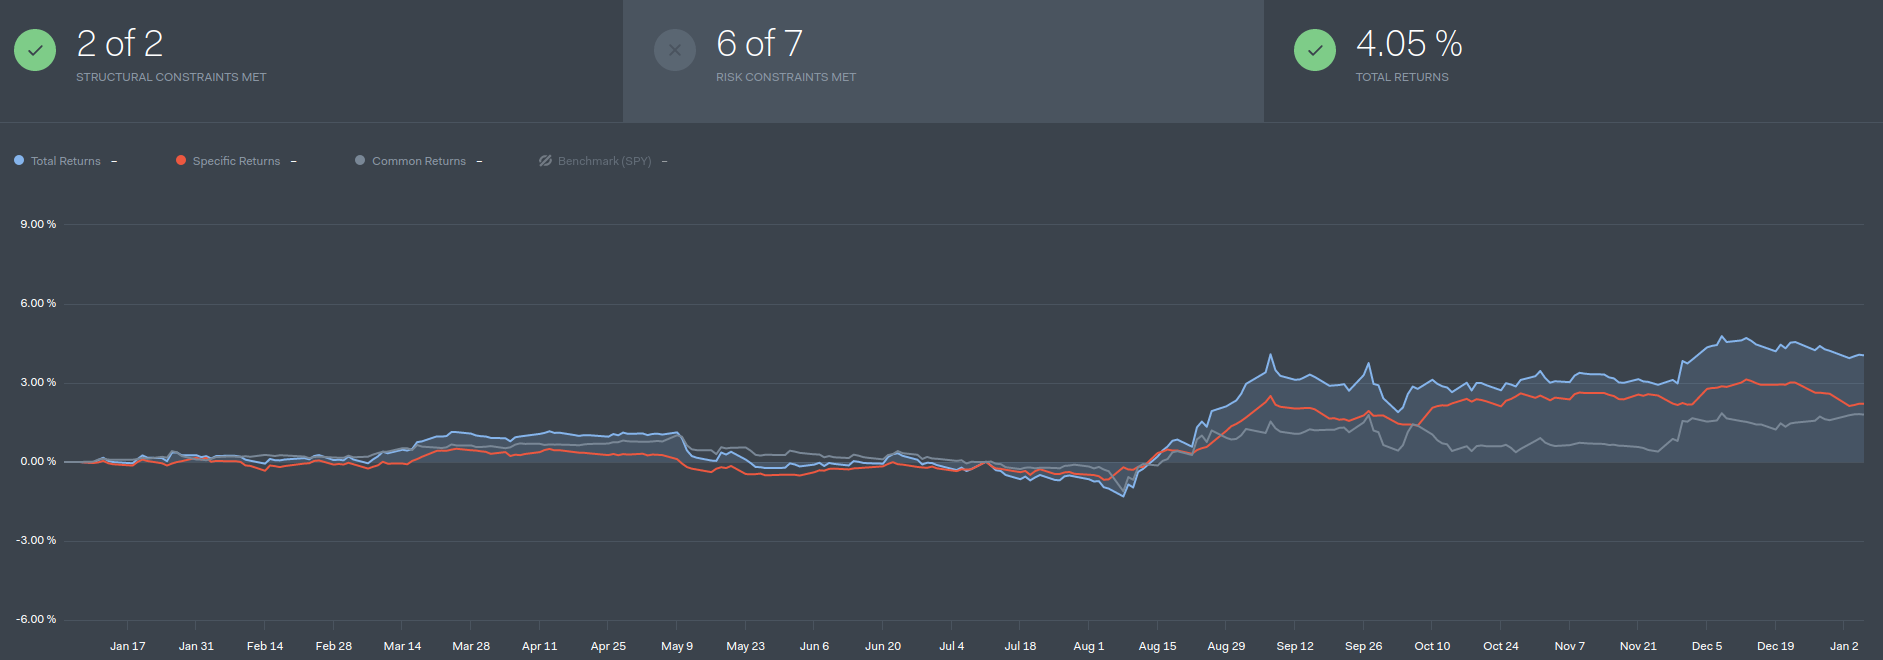
\includegraphics[width=1.1\linewidth]{linea_base}
	\caption{Resultados de la linea base del algoritmo}
	\label{fig:lineabase}
\end{figure}

En el siguiente experimento hacemos que el algoritmo empiece desde el miercoles en lugar de una vez a la semana lo hacemos todos los dias, y hacemos que el algoritmo solo pueda ver 2 dias hacia atras. Con esto obtenemos la Figura \ref{fig:experimento1} que indica que actualizar tan rapidamente los stocks con tan poca información no es buena idea. \\

 \begin{figure}[h]
	\centering
	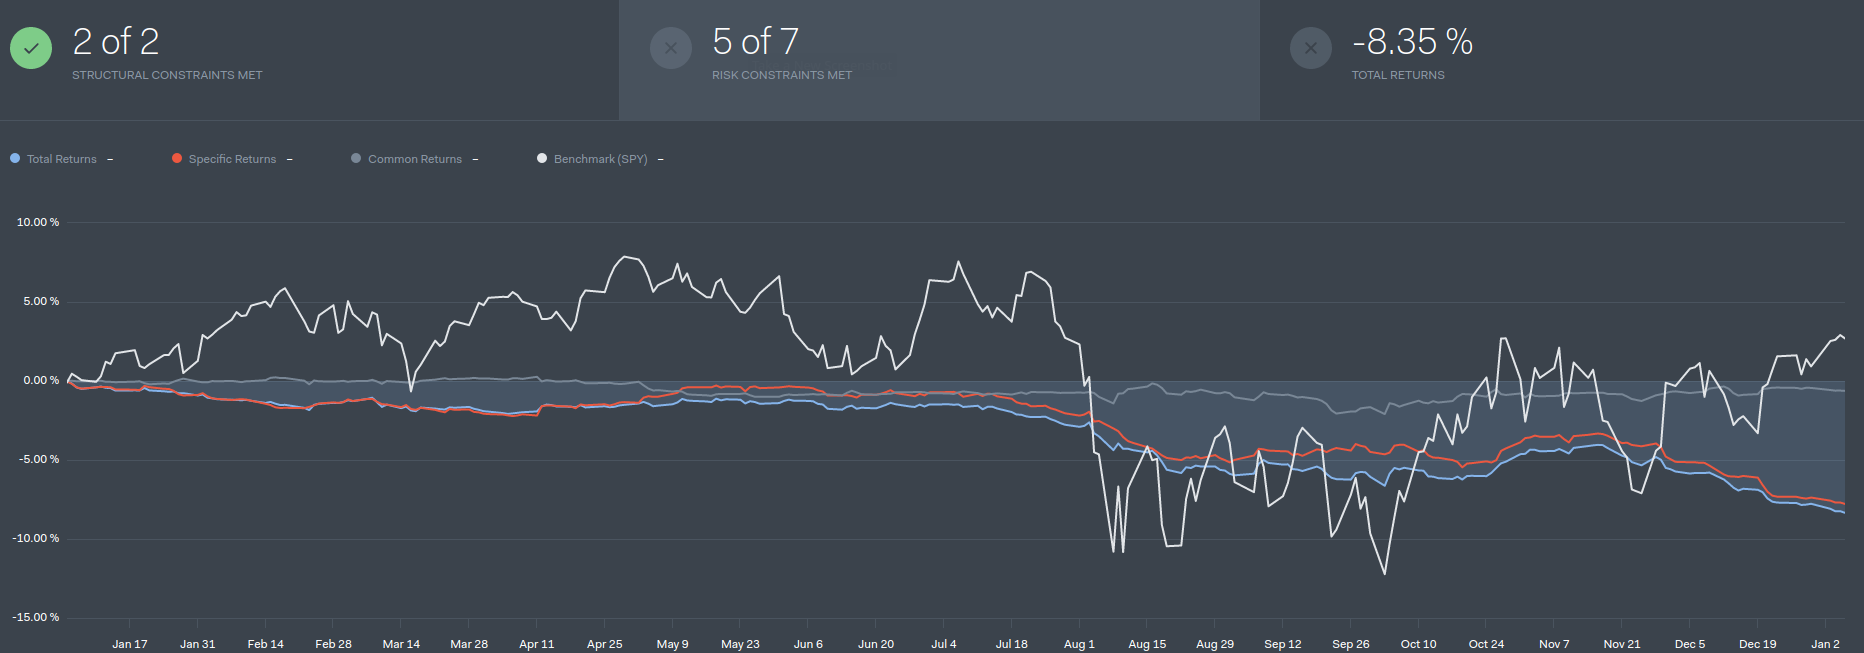
\includegraphics[width=1.1\linewidth]{experimento_1}
	\caption{Resultados del primer experimento}
	\label{fig:experimento1}
\end{figure}
Para el siguiente experimento consideramos que el algoritmo se ejecute cada semana con información de 6 dias y que además aumente el \verb|MAX_POSITION_CONCENTRATION| a $0.05$ , los resultados que se indican en la Figura \ref{fig:experimento2} indican que nuestras perdidas y nuestras ganancias son más grandes a las de la linea base, es un algoritmo más "agresivo".\\


\begin{figure}[h]
	\centering
	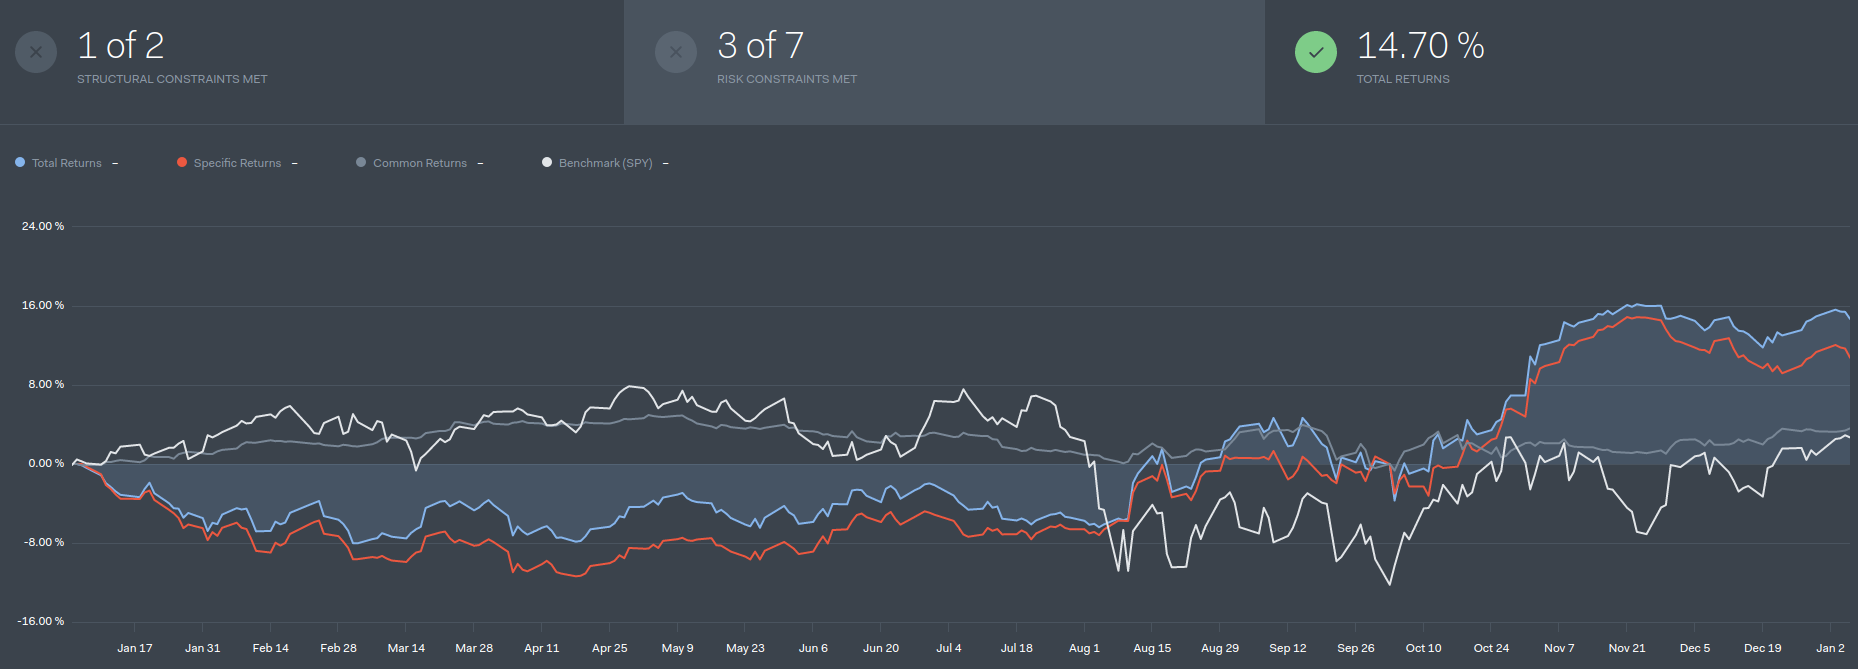
\includegraphics[width=1.1\linewidth]{experimento_2}
	\caption{Resultados del segundo experimento }
	\label{fig:experimento2}
\end{figure}

Ahora deberíamos pensar en que el algoritmo tuvo poca información en el primer experimento. Por tanto vamos a rebalancear teniendo en cuenta que se actualiza todos los dias pero con más información de por medio, es decir en vez de dos días le vamos a dar 10 y dejar el resto de variables como en el anterior experimento.  Los resultados se pueden ver en la Figura \ref{fig:experimento3}, muestran que no solo se minimizan las perdidas tambien se maximizan las ganancias. \\


\begin{figure}[h]
	\centering
	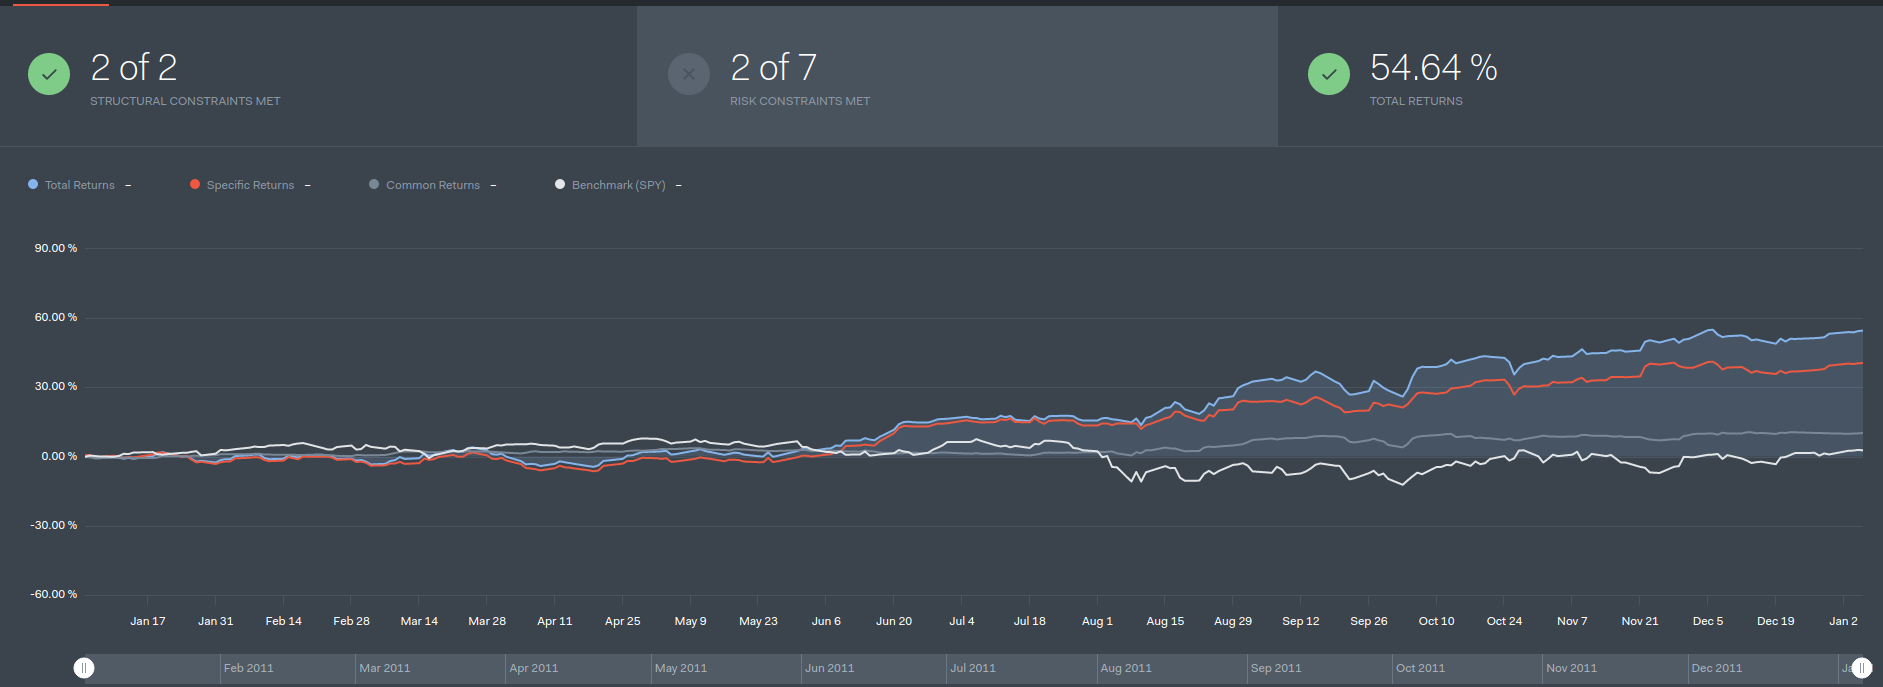
\includegraphics[width=1.1\linewidth]{experimento_3}
	\caption{Resultados del experimento 3}
	\label{fig:experimento3}
\end{figure}

Para este experimento modificamos la forma en la que se toman los percentiles de altos y bajos para ir largo y corto respectivamente. Los bajos los dejamos en 13\% y los altos los dejamos en 7\%. El  experimento que se muestra en la Figura \ref{fig:experimento4} evidencia que el cambio no es significativo y no hace gran diferencia comparado a los anteriores. \\
\begin{figure}
	\centering
	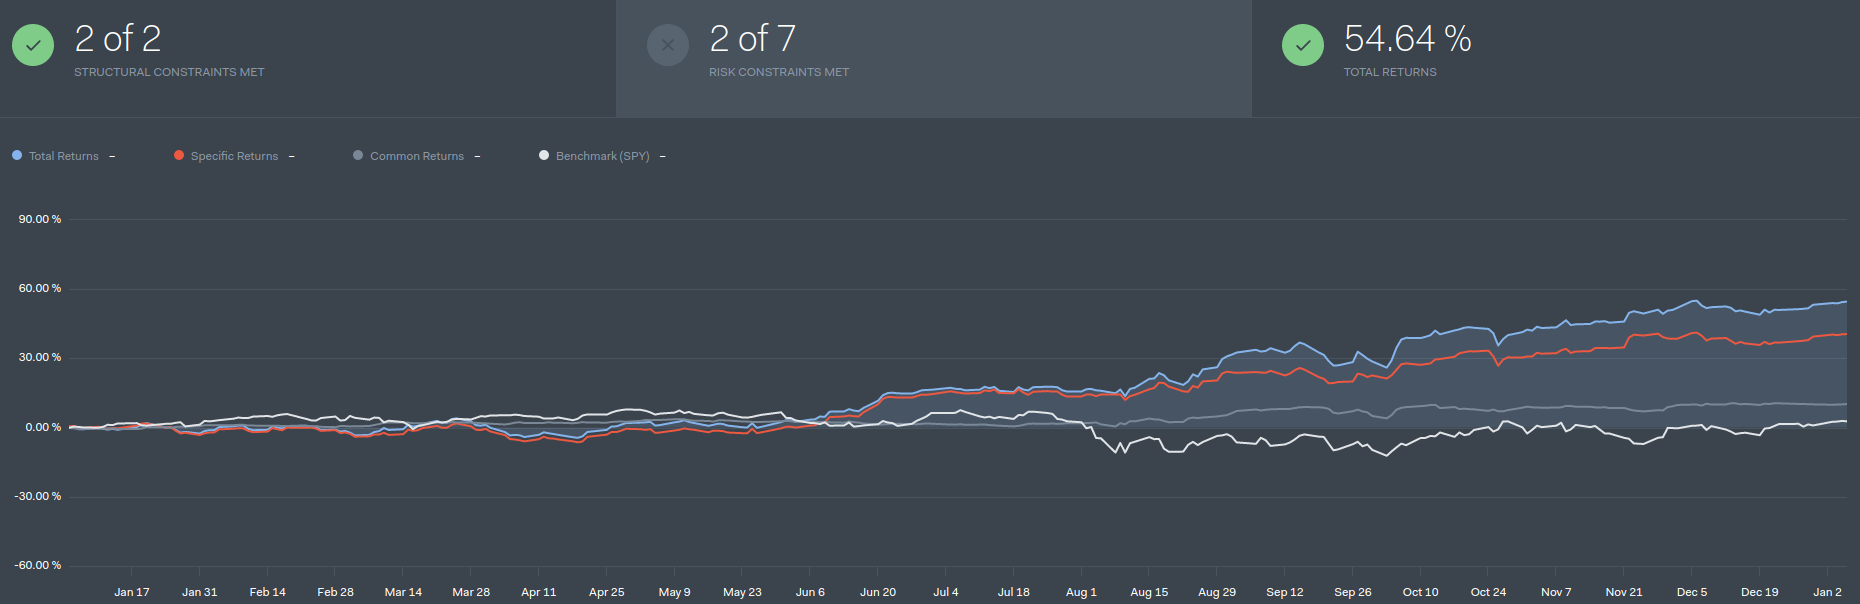
\includegraphics[width=1.1\linewidth]{experimento_4}
	\caption{Resultados cuarto experimento }
	\label{fig:experimento4}
\end{figure}
Para el último experimento consideramos que debemos cambiar el universo así que en vez de tomar todo el universo de las acciones tomamos únicamente las 1000 con mejor "revenue". De esta forma tenemos el quinto experimento que nos muestra que el algoritmo es muy similar SPY y que de hecho se pierde dinero.
\begin{figure}
	\centering
	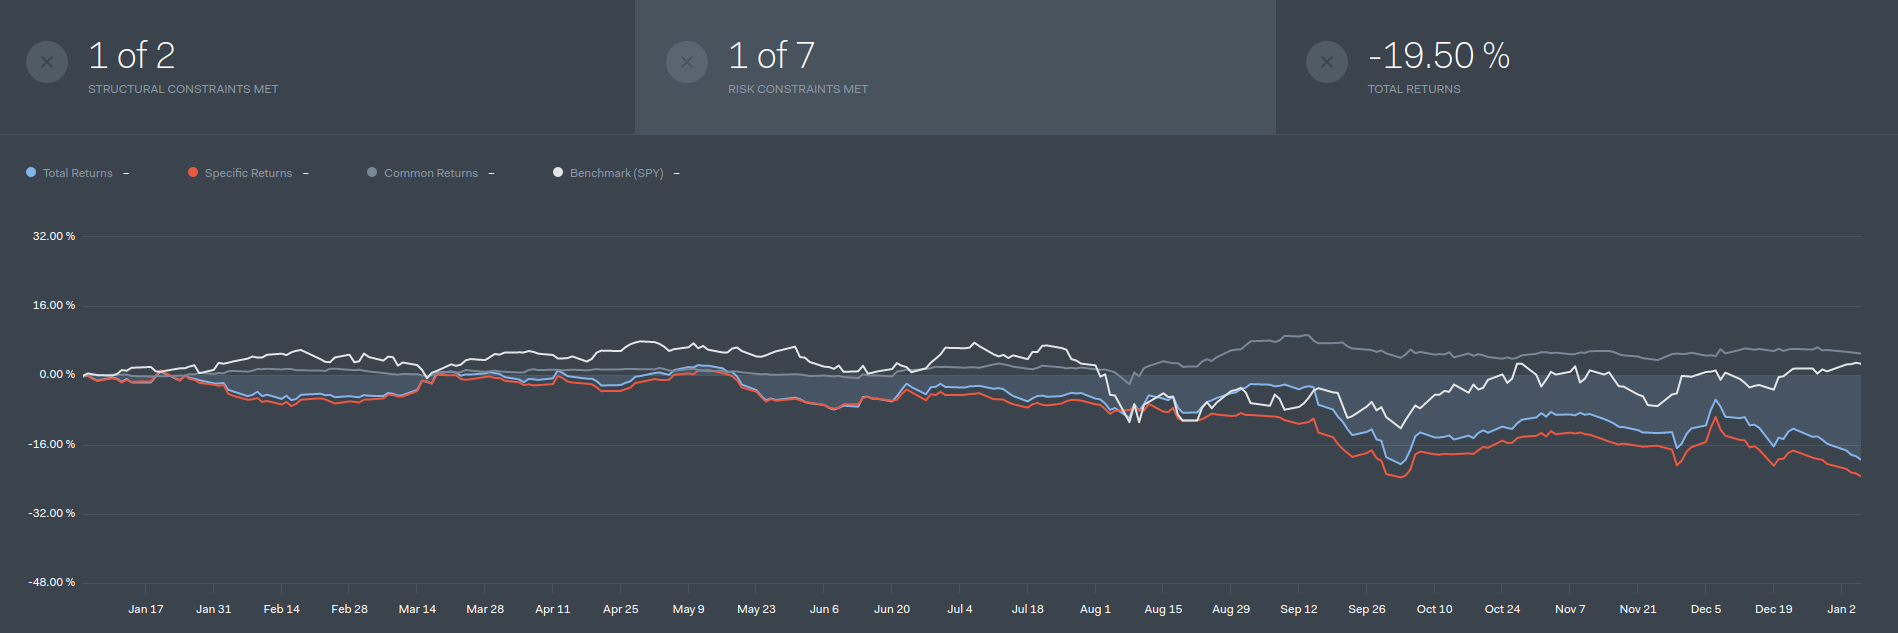
\includegraphics[width=1.1\linewidth]{experimento_5}
	\caption{Resultados del quinto experimento}
	\label{fig:experimento5}
\end{figure}
\\

El código con el cual se termina y que da un resultado de 54\% de ganancia es :
\lstinputlisting[language=Python]{algoritmo.py}


Por último para analizar las acciones vendidas tomamos BKI de la cual se compraron $1500$USD el primero de enero de 2011. En la Figura \ref{fig:compra}  se puede notar que la acción crece durante el periodo que le sigue a la compra usando yahoo Finance para obtener la información. Además contamos con la información provista para RDN con la cual se vendió $ 1700$ USD y se puede notar como disminuyeron de precio.\\


\begin{figure}
	\centering
	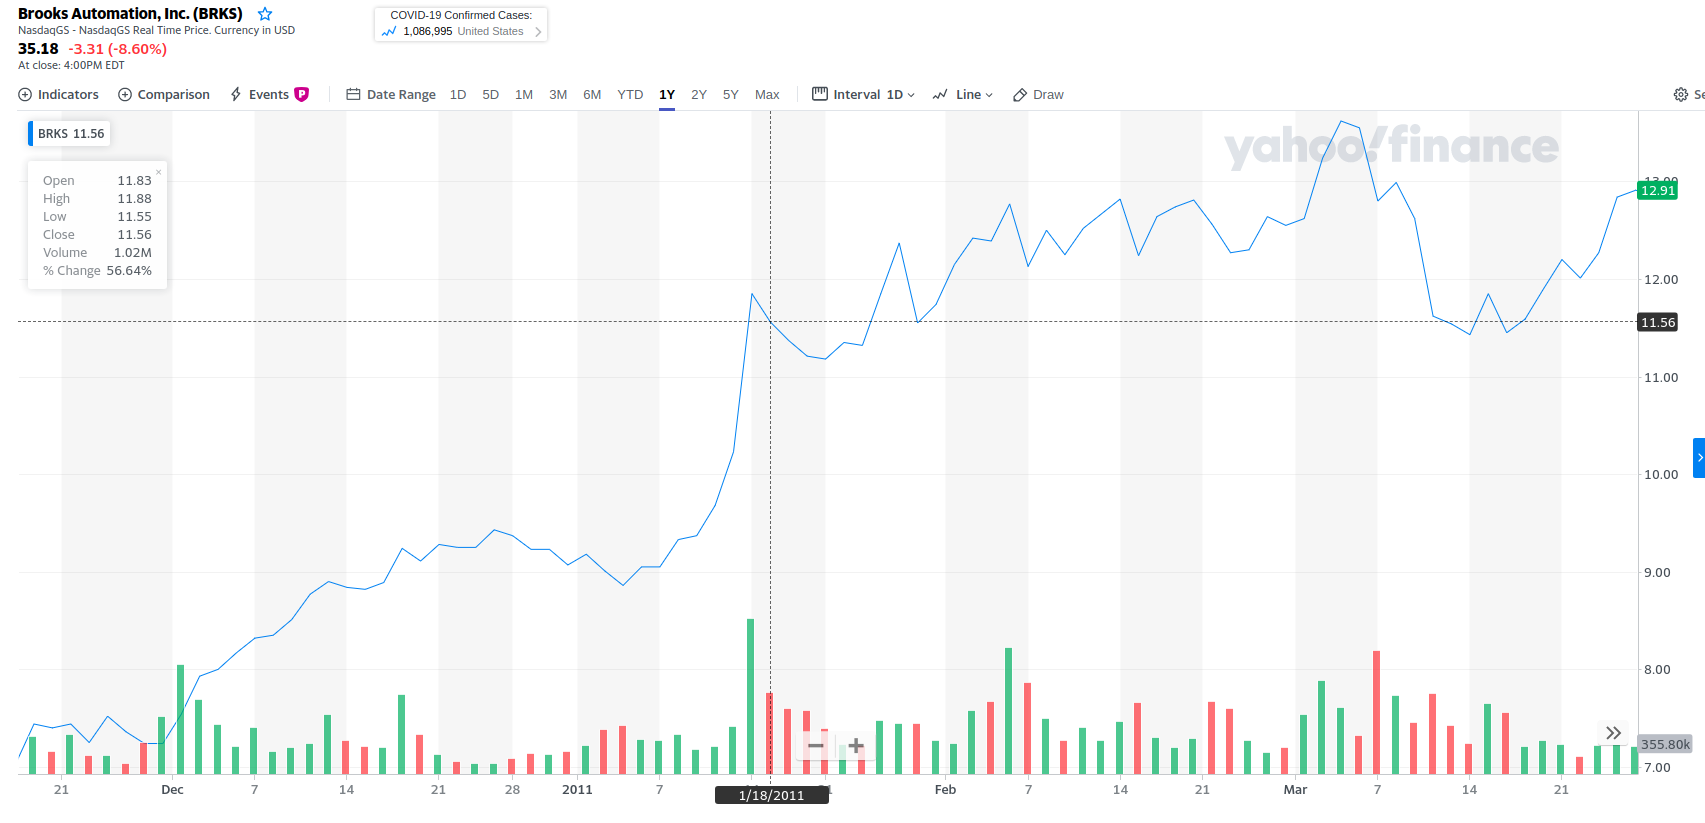
\includegraphics[width=1\linewidth]{compra}
	\caption{Comportamiento de una acción que se compro usando en el algoritmo}
	\label{fig:compra}
\end{figure}
\begin{figure}
	\centering
	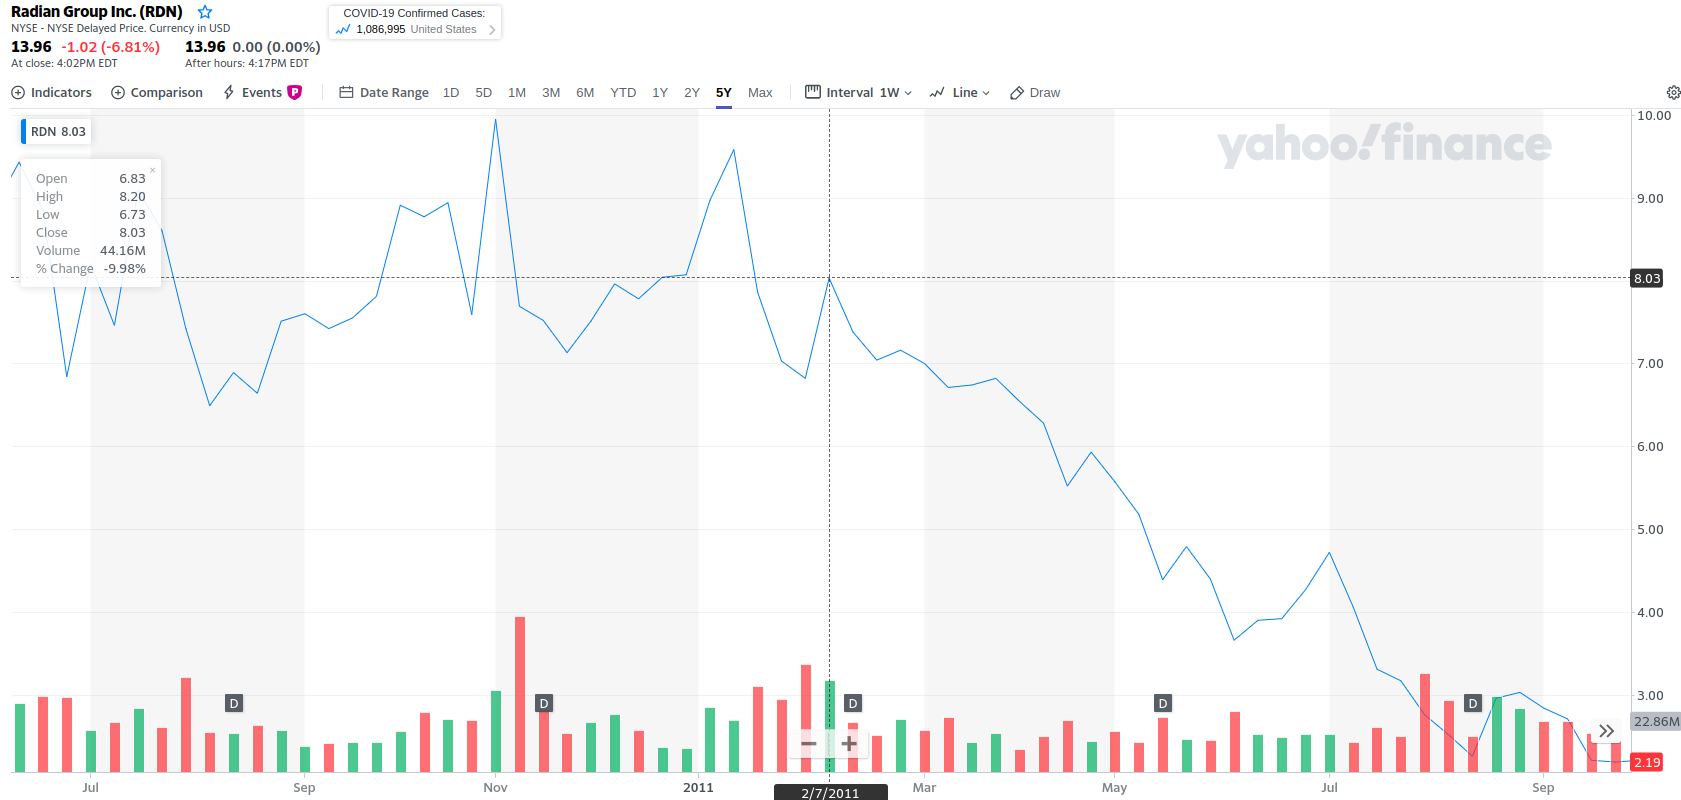
\includegraphics[width=1\linewidth]{venta}
	\caption{Comportamiento de una acción que se vendió usando en el algoritmo}
	\label{fig:venta}
\end{figure}





\end{document}